\section{Mode Diagram}

REQ\ref{R1} states The \emph{controller} shall operate in one of four modes: \emph{off}, \emph{init}, \emph{normal} and \emph{fail}, shown in Fig.~\ref{fig:sc}. As shown in the figure, the Isolette will begin in the \emph{off} mode, and will enter \emph{init} mode when the nurse flips \mv{sw} into the \emph{on} position. The Isolette will only be able to move from the \emph{init} mode ot the \emph{normal} mode if it is properly configured such that the desired range is valid and not overlapping with the alarm levels, and both the sensors and operator controls are working (see REQ\ref{R6}).
Once inside the \emph{normal} mode, the controller will move to the \emph{fail} mode if either the controls or sensor fails, as specified in REQ\ref{R5}, and will only return to the \emph{normal} mode once they are both working correctly (REQ\ref{R7}). In any of these states, if the nurse switches \mv{sw} to \emph{off} the controller will switch to the off mode (REQ\ref{R8}).

\begin{figure}[!htb]
\begin{mdframed}
\begin{center}
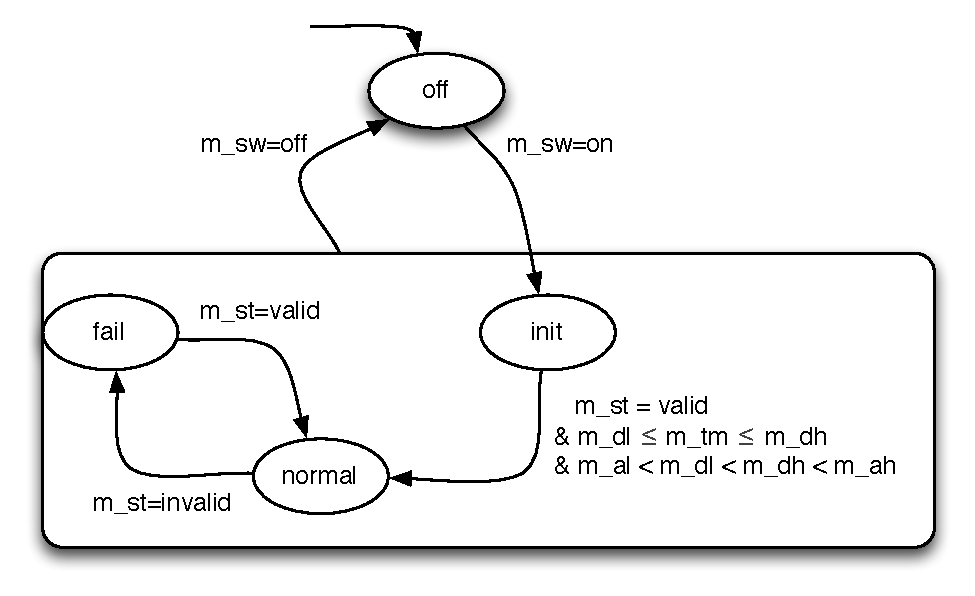
\includegraphics[width=.9\textwidth]{pics/mode-statechart.pdf}
\end{center}
\end{mdframed}
\caption{Statechart for the modes variable \cv{md}}
\label{fig:sc}
\end{figure}